\documentclass[twoside]{book}

% Packages required by doxygen
\usepackage{calc}
\usepackage{doxygen}
\usepackage{graphicx}
\usepackage[utf8]{inputenc}
\usepackage{makeidx}
\usepackage{multicol}
\usepackage{multirow}
\usepackage{textcomp}
\usepackage[table]{xcolor}

% Font selection
\usepackage[T1]{fontenc}
\usepackage{mathptmx}
\usepackage[scaled=.90]{helvet}
\usepackage{courier}
\usepackage{amssymb}
\usepackage{sectsty}
\renewcommand{\familydefault}{\sfdefault}
\allsectionsfont{%
  \fontseries{bc}\selectfont%
  \color{darkgray}%
}
\renewcommand{\DoxyLabelFont}{%
  \fontseries{bc}\selectfont%
  \color{darkgray}%
}

% Page & text layout
\usepackage{geometry}
\geometry{%
  a4paper,%
  top=2.5cm,%
  bottom=2.5cm,%
  left=2.5cm,%
  right=2.5cm%
}
\tolerance=750
\hfuzz=15pt
\hbadness=750
\setlength{\emergencystretch}{15pt}
\setlength{\parindent}{0cm}
\setlength{\parskip}{0.2cm}
\makeatletter
\renewcommand{\paragraph}{%
  \@startsection{paragraph}{4}{0ex}{-1.0ex}{1.0ex}{%
    \normalfont\normalsize\bfseries\SS@parafont%
  }%
}
\renewcommand{\subparagraph}{%
  \@startsection{subparagraph}{5}{0ex}{-1.0ex}{1.0ex}{%
    \normalfont\normalsize\bfseries\SS@subparafont%
  }%
}
\makeatother

% Headers & footers
\usepackage{fancyhdr}
\pagestyle{fancyplain}
\fancyhead[LE]{\fancyplain{}{\bfseries\thepage}}
\fancyhead[CE]{\fancyplain{}{}}
\fancyhead[RE]{\fancyplain{}{\bfseries\leftmark}}
\fancyhead[LO]{\fancyplain{}{\bfseries\rightmark}}
\fancyhead[CO]{\fancyplain{}{}}
\fancyhead[RO]{\fancyplain{}{\bfseries\thepage}}
\fancyfoot[LE]{\fancyplain{}{}}
\fancyfoot[CE]{\fancyplain{}{}}
\fancyfoot[RE]{\fancyplain{}{\bfseries\scriptsize Generated on Mon Jun 26 2017 10\-:47\-:21 for Shine Client by Doxygen }}
\fancyfoot[LO]{\fancyplain{}{\bfseries\scriptsize Generated on Mon Jun 26 2017 10\-:47\-:21 for Shine Client by Doxygen }}
\fancyfoot[CO]{\fancyplain{}{}}
\fancyfoot[RO]{\fancyplain{}{}}
\renewcommand{\footrulewidth}{0.4pt}
\renewcommand{\chaptermark}[1]{%
  \markboth{#1}{}%
}
\renewcommand{\sectionmark}[1]{%
  \markright{\thesection\ #1}%
}

% Indices & bibliography
\usepackage{natbib}
\usepackage[titles]{tocloft}
\setcounter{tocdepth}{3}
\setcounter{secnumdepth}{5}
\makeindex

% Hyperlinks (required, but should be loaded last)
\usepackage{ifpdf}
\ifpdf
  \usepackage[pdftex,pagebackref=true]{hyperref}
\else
  \usepackage[ps2pdf,pagebackref=true]{hyperref}
\fi
\hypersetup{%
  colorlinks=true,%
  linkcolor=blue,%
  citecolor=blue,%
  unicode%
}

% Custom commands
\newcommand{\clearemptydoublepage}{%
  \newpage{\pagestyle{empty}\cleardoublepage}%
}


%===== C O N T E N T S =====

\begin{document}

% Titlepage & ToC
\hypersetup{pageanchor=false}
\pagenumbering{roman}
\begin{titlepage}
\vspace*{7cm}
\begin{center}%
{\Large Shine Client }\\
\vspace*{1cm}
{\large Generated by Doxygen 1.8.6}\\
\vspace*{0.5cm}
{\small Mon Jun 26 2017 10:47:21}\\
\end{center}
\end{titlepage}
\clearemptydoublepage
\tableofcontents
\clearemptydoublepage
\pagenumbering{arabic}
\hypersetup{pageanchor=true}

%--- Begin generated contents ---
\chapter{Class Index}
\section{Class List}
Here are the classes, structs, unions and interfaces with brief descriptions\-:\begin{DoxyCompactList}
\item\contentsline{section}{\hyperlink{structARC__STRUCT}{A\-R\-C\-\_\-\-S\-T\-R\-U\-C\-T} }{\pageref{structARC__STRUCT}}{}
\item\contentsline{section}{\hyperlink{structCF__DATA}{C\-F\-\_\-\-D\-A\-T\-A} }{\pageref{structCF__DATA}}{}
\item\contentsline{section}{\hyperlink{structConfig}{Config} }{\pageref{structConfig}}{}
\item\contentsline{section}{\hyperlink{structDATA__MATRIX}{D\-A\-T\-A\-\_\-\-M\-A\-T\-R\-I\-X} }{\pageref{structDATA__MATRIX}}{}
\item\contentsline{section}{\hyperlink{structHEADER__TRANSMISSION}{H\-E\-A\-D\-E\-R\-\_\-\-T\-R\-A\-N\-S\-M\-I\-S\-S\-I\-O\-N} }{\pageref{structHEADER__TRANSMISSION}}{}
\item\contentsline{section}{\hyperlink{structLIST__STRUCT}{L\-I\-S\-T\-\_\-\-S\-T\-R\-U\-C\-T} }{\pageref{structLIST__STRUCT}}{}
\item\contentsline{section}{\hyperlink{structNODE__LIST__STRUCT}{N\-O\-D\-E\-\_\-\-L\-I\-S\-T\-\_\-\-S\-T\-R\-U\-C\-T} }{\pageref{structNODE__LIST__STRUCT}}{}
\item\contentsline{section}{\hyperlink{structNODE__STRUCT}{N\-O\-D\-E\-\_\-\-S\-T\-R\-U\-C\-T} }{\pageref{structNODE__STRUCT}}{}
\item\contentsline{section}{\hyperlink{structNODE__SUBSET__STRUCT}{N\-O\-D\-E\-\_\-\-S\-U\-B\-S\-E\-T\-\_\-\-S\-T\-R\-U\-C\-T} }{\pageref{structNODE__SUBSET__STRUCT}}{}
\item\contentsline{section}{\hyperlink{structNODO}{N\-O\-D\-O} }{\pageref{structNODO}}{}
\item\contentsline{section}{\hyperlink{structRANDOM__LIST}{R\-A\-N\-D\-O\-M\-\_\-\-L\-I\-S\-T} }{\pageref{structRANDOM__LIST}}{}
\item\contentsline{section}{\hyperlink{structRCL__LIST__STRUCT}{R\-C\-L\-\_\-\-L\-I\-S\-T\-\_\-\-S\-T\-R\-U\-C\-T} }{\pageref{structRCL__LIST__STRUCT}}{}
\item\contentsline{section}{\hyperlink{structSUBSET__STRUCT}{S\-U\-B\-S\-E\-T\-\_\-\-S\-T\-R\-U\-C\-T} }{\pageref{structSUBSET__STRUCT}}{}
\end{DoxyCompactList}

\chapter{File Index}
\section{File List}
Here is a list of all documented files with brief descriptions\-:\begin{DoxyCompactList}
\item\contentsline{section}{\hyperlink{client_8cpp}{client.\-cpp} \\*The main file to use the client }{\pageref{client_8cpp}}{}
\item\contentsline{section}{\hyperlink{CodingDecodingData_8cpp}{Coding\-Decoding\-Data.\-cpp} \\*The file that perform the decoding }{\pageref{CodingDecodingData_8cpp}}{}
\item\contentsline{section}{{\bfseries Coding\-Decoding\-Data.\-h} }{\pageref{CodingDecodingData_8h}}{}
\item\contentsline{section}{{\bfseries Data\-Definition.\-h} }{\pageref{DataDefinition_8h}}{}
\item\contentsline{section}{\hyperlink{LibShine_8cpp}{Lib\-Shine.\-cpp} \\*The file to load configuration file }{\pageref{LibShine_8cpp}}{}
\item\contentsline{section}{{\bfseries Lib\-Shine.\-h} }{\pageref{LibShine_8h}}{}
\item\contentsline{section}{\hyperlink{utilityForTesting_8cpp}{utility\-For\-Testing.\-cpp} \\*A file containing utility function }{\pageref{utilityForTesting_8cpp}}{}
\item\contentsline{section}{{\bfseries utility\-For\-Testing.\-h} }{\pageref{utilityForTesting_8h}}{}
\end{DoxyCompactList}

\chapter{Class Documentation}
\hypertarget{structARC__STRUCT}{\section{A\-R\-C\-\_\-\-S\-T\-R\-U\-C\-T Struct Reference}
\label{structARC__STRUCT}\index{A\-R\-C\-\_\-\-S\-T\-R\-U\-C\-T@{A\-R\-C\-\_\-\-S\-T\-R\-U\-C\-T}}
}


{\ttfamily \#include $<$Data\-Definition.\-h$>$}

\subsection*{Public Attributes}
\begin{DoxyCompactItemize}
\item 
int \hyperlink{structARC__STRUCT_aed399ecc75eab66d87a638f46b12fff1}{adj}
\end{DoxyCompactItemize}


\subsection{Member Data Documentation}
\hypertarget{structARC__STRUCT_aed399ecc75eab66d87a638f46b12fff1}{\index{A\-R\-C\-\_\-\-S\-T\-R\-U\-C\-T@{A\-R\-C\-\_\-\-S\-T\-R\-U\-C\-T}!adj@{adj}}
\index{adj@{adj}!ARC_STRUCT@{A\-R\-C\-\_\-\-S\-T\-R\-U\-C\-T}}
\subsubsection[{adj}]{\setlength{\rightskip}{0pt plus 5cm}int A\-R\-C\-\_\-\-S\-T\-R\-U\-C\-T\-::adj}}\label{structARC__STRUCT_aed399ecc75eab66d87a638f46b12fff1}


The documentation for this struct was generated from the following file\-:\begin{DoxyCompactItemize}
\item 
\hyperlink{DataDefinition_8h}{Data\-Definition.\-h}\end{DoxyCompactItemize}

\hypertarget{structCF__DATA}{\section{C\-F\-\_\-\-D\-A\-T\-A Struct Reference}
\label{structCF__DATA}\index{C\-F\-\_\-\-D\-A\-T\-A@{C\-F\-\_\-\-D\-A\-T\-A}}
}
\subsection*{Public Attributes}
\begin{DoxyCompactItemize}
\item 
\hypertarget{structCF__DATA_a33150ceb864cb8ff1fcf8bfbb2d01efe}{int $\ast$$\ast$ {\bfseries Matrix\-\_\-\-Adj}}\label{structCF__DATA_a33150ceb864cb8ff1fcf8bfbb2d01efe}

\item 
\hypertarget{structCF__DATA_aa790d2fc6304b584e3d6a5afb95cf5c4}{\hyperlink{structNODO}{nodo} $\ast$ {\bfseries nodes}}\label{structCF__DATA_aa790d2fc6304b584e3d6a5afb95cf5c4}

\item 
\hypertarget{structCF__DATA_a50c302ea5a7570881d844eb0b2a6c930}{int {\bfseries n\-\_\-nodi}}\label{structCF__DATA_a50c302ea5a7570881d844eb0b2a6c930}

\item 
\hypertarget{structCF__DATA_a21b2ca110fc0b01950a783ef9e9c2628}{int $\ast$$\ast$$\ast$ {\bfseries Ind}}\label{structCF__DATA_a21b2ca110fc0b01950a783ef9e9c2628}

\end{DoxyCompactItemize}


The documentation for this struct was generated from the following file\-:\begin{DoxyCompactItemize}
\item 
Data\-Definition.\-h\end{DoxyCompactItemize}

\hypertarget{structConfig}{\section{Config Struct Reference}
\label{structConfig}\index{Config@{Config}}
}
\subsection*{Public Attributes}
\begin{DoxyCompactItemize}
\item 
\hypertarget{structConfig_afc8ae6cab0cd9fa1ea54ca13bacd56ea}{int {\bfseries hello\-\_\-port}}\label{structConfig_afc8ae6cab0cd9fa1ea54ca13bacd56ea}

\item 
\hypertarget{structConfig_a2b1264000682b7de201becb6e6fb919d}{char $\ast$ {\bfseries hello\-\_\-group} = new char\mbox{[}10\mbox{]}}\label{structConfig_a2b1264000682b7de201becb6e6fb919d}

\item 
\hypertarget{structConfig_a4a5c2783f6aa2283fb3343082bff5ef7}{int {\bfseries n\-Files}}\label{structConfig_a4a5c2783f6aa2283fb3343082bff5ef7}

\item 
\hypertarget{structConfig_a0a3293605217709540e386fb81eca8bb}{string {\bfseries path\-Repo}}\label{structConfig_a0a3293605217709540e386fb81eca8bb}

\item 
\hypertarget{structConfig_acde368864b2d950bfde458664732a3c6}{int {\bfseries max\-Size}}\label{structConfig_acde368864b2d950bfde458664732a3c6}

\end{DoxyCompactItemize}


The documentation for this struct was generated from the following file\-:\begin{DoxyCompactItemize}
\item 
Lib\-Shine.\-h\end{DoxyCompactItemize}

\hypertarget{structDATA__MATRIX}{\section{D\-A\-T\-A\-\_\-\-M\-A\-T\-R\-I\-X Struct Reference}
\label{structDATA__MATRIX}\index{D\-A\-T\-A\-\_\-\-M\-A\-T\-R\-I\-X@{D\-A\-T\-A\-\_\-\-M\-A\-T\-R\-I\-X}}
}
\subsection*{Public Attributes}
\begin{DoxyCompactItemize}
\item 
\hypertarget{structDATA__MATRIX_aae6daea8805e8718aa68a84bcca6241b}{int {\bfseries n\-\_\-utenti}}\label{structDATA__MATRIX_aae6daea8805e8718aa68a84bcca6241b}

\item 
\hypertarget{structDATA__MATRIX_a4dabab55b019bad68745b2017beca72f}{int {\bfseries m\-\_\-files}}\label{structDATA__MATRIX_a4dabab55b019bad68745b2017beca72f}

\item 
\hypertarget{structDATA__MATRIX_a2d20067a548ed52d36fbc33ea8be6920}{int {\bfseries b\-\_\-chunks}}\label{structDATA__MATRIX_a2d20067a548ed52d36fbc33ea8be6920}

\item 
\hypertarget{structDATA__MATRIX_ab84fa0383965f21e5169de993040734a}{int $\ast$$\ast$$\ast$ {\bfseries Ind}}\label{structDATA__MATRIX_ab84fa0383965f21e5169de993040734a}

\item 
\hypertarget{structDATA__MATRIX_a6cc2252dd6e2e65dd098c0ded22a75a9}{int $\ast$ {\bfseries Q}}\label{structDATA__MATRIX_a6cc2252dd6e2e65dd098c0ded22a75a9}

\item 
\hypertarget{structDATA__MATRIX_afddbea5ee6d0ab5d894b4ac1dc79681c}{int $\ast$$\ast$ {\bfseries Q\-\_\-chuncks}}\label{structDATA__MATRIX_afddbea5ee6d0ab5d894b4ac1dc79681c}

\end{DoxyCompactItemize}


The documentation for this struct was generated from the following file\-:\begin{DoxyCompactItemize}
\item 
Data\-Definition.\-h\end{DoxyCompactItemize}

\hypertarget{structHEADER__TRANSMISSION}{\section{H\-E\-A\-D\-E\-R\-\_\-\-T\-R\-A\-N\-S\-M\-I\-S\-S\-I\-O\-N Struct Reference}
\label{structHEADER__TRANSMISSION}\index{H\-E\-A\-D\-E\-R\-\_\-\-T\-R\-A\-N\-S\-M\-I\-S\-S\-I\-O\-N@{H\-E\-A\-D\-E\-R\-\_\-\-T\-R\-A\-N\-S\-M\-I\-S\-S\-I\-O\-N}}
}


{\ttfamily \#include $<$Data\-Definition.\-h$>$}

\subsection*{Public Attributes}
\begin{DoxyCompactItemize}
\item 
int \hyperlink{structHEADER__TRANSMISSION_a74de1a2343e132bf28eb6e83b4601d34}{padding}
\begin{DoxyCompactList}\small\item\em (1 byte) is used to identify the last chunk for requested file. \end{DoxyCompactList}\item 
int \hyperlink{structHEADER__TRANSMISSION_abee64c077b815db300d99d1e2a273af7}{num\-\_\-chunks}
\begin{DoxyCompactList}\small\item\em define how many chunks are send together. \end{DoxyCompactList}\item 
vector$<$ int $>$ \hyperlink{structHEADER__TRANSMISSION_ae1d8e1fcc8178250b212f77325022424}{id\-\_\-utenti}
\begin{DoxyCompactList}\small\item\em a list of users identifiers. \end{DoxyCompactList}\item 
vector$<$ int $>$ \hyperlink{structHEADER__TRANSMISSION_a7d6396f1a9a35defc1b44e00c663b412}{id\-\_\-files}
\begin{DoxyCompactList}\small\item\em a list of files identifiers. \end{DoxyCompactList}\item 
vector$<$ int $>$ \hyperlink{structHEADER__TRANSMISSION_a3fa5dd88f6fc08f8c64eaee74408ce0e}{id\-\_\-chunks}
\begin{DoxyCompactList}\small\item\em a list of chunks identifiers. \end{DoxyCompactList}\item 
vector$<$ int $>$ \hyperlink{structHEADER__TRANSMISSION_a08672f07c936f6bc4127fe255ea0ce7e}{size\-\_\-package}
\begin{DoxyCompactList}\small\item\em a list of the sizes of every chunk send. This list is useful when padding is 1. \end{DoxyCompactList}\item 
int \hyperlink{structHEADER__TRANSMISSION_a0654a40688064ef0925896891de48b43}{size\-Tot}
\begin{DoxyCompactList}\small\item\em Total package size. \end{DoxyCompactList}\end{DoxyCompactItemize}


\subsection{Member Data Documentation}
\hypertarget{structHEADER__TRANSMISSION_a3fa5dd88f6fc08f8c64eaee74408ce0e}{\index{H\-E\-A\-D\-E\-R\-\_\-\-T\-R\-A\-N\-S\-M\-I\-S\-S\-I\-O\-N@{H\-E\-A\-D\-E\-R\-\_\-\-T\-R\-A\-N\-S\-M\-I\-S\-S\-I\-O\-N}!id\-\_\-chunks@{id\-\_\-chunks}}
\index{id\-\_\-chunks@{id\-\_\-chunks}!HEADER_TRANSMISSION@{H\-E\-A\-D\-E\-R\-\_\-\-T\-R\-A\-N\-S\-M\-I\-S\-S\-I\-O\-N}}
\subsubsection[{id\-\_\-chunks}]{\setlength{\rightskip}{0pt plus 5cm}H\-E\-A\-D\-E\-R\-\_\-\-T\-R\-A\-N\-S\-M\-I\-S\-S\-I\-O\-N\-::id\-\_\-chunks}}\label{structHEADER__TRANSMISSION_a3fa5dd88f6fc08f8c64eaee74408ce0e}


a list of chunks identifiers. 

\hypertarget{structHEADER__TRANSMISSION_a7d6396f1a9a35defc1b44e00c663b412}{\index{H\-E\-A\-D\-E\-R\-\_\-\-T\-R\-A\-N\-S\-M\-I\-S\-S\-I\-O\-N@{H\-E\-A\-D\-E\-R\-\_\-\-T\-R\-A\-N\-S\-M\-I\-S\-S\-I\-O\-N}!id\-\_\-files@{id\-\_\-files}}
\index{id\-\_\-files@{id\-\_\-files}!HEADER_TRANSMISSION@{H\-E\-A\-D\-E\-R\-\_\-\-T\-R\-A\-N\-S\-M\-I\-S\-S\-I\-O\-N}}
\subsubsection[{id\-\_\-files}]{\setlength{\rightskip}{0pt plus 5cm}H\-E\-A\-D\-E\-R\-\_\-\-T\-R\-A\-N\-S\-M\-I\-S\-S\-I\-O\-N\-::id\-\_\-files}}\label{structHEADER__TRANSMISSION_a7d6396f1a9a35defc1b44e00c663b412}


a list of files identifiers. 

\hypertarget{structHEADER__TRANSMISSION_ae1d8e1fcc8178250b212f77325022424}{\index{H\-E\-A\-D\-E\-R\-\_\-\-T\-R\-A\-N\-S\-M\-I\-S\-S\-I\-O\-N@{H\-E\-A\-D\-E\-R\-\_\-\-T\-R\-A\-N\-S\-M\-I\-S\-S\-I\-O\-N}!id\-\_\-utenti@{id\-\_\-utenti}}
\index{id\-\_\-utenti@{id\-\_\-utenti}!HEADER_TRANSMISSION@{H\-E\-A\-D\-E\-R\-\_\-\-T\-R\-A\-N\-S\-M\-I\-S\-S\-I\-O\-N}}
\subsubsection[{id\-\_\-utenti}]{\setlength{\rightskip}{0pt plus 5cm}H\-E\-A\-D\-E\-R\-\_\-\-T\-R\-A\-N\-S\-M\-I\-S\-S\-I\-O\-N\-::id\-\_\-utenti}}\label{structHEADER__TRANSMISSION_ae1d8e1fcc8178250b212f77325022424}


a list of users identifiers. 

\hypertarget{structHEADER__TRANSMISSION_abee64c077b815db300d99d1e2a273af7}{\index{H\-E\-A\-D\-E\-R\-\_\-\-T\-R\-A\-N\-S\-M\-I\-S\-S\-I\-O\-N@{H\-E\-A\-D\-E\-R\-\_\-\-T\-R\-A\-N\-S\-M\-I\-S\-S\-I\-O\-N}!num\-\_\-chunks@{num\-\_\-chunks}}
\index{num\-\_\-chunks@{num\-\_\-chunks}!HEADER_TRANSMISSION@{H\-E\-A\-D\-E\-R\-\_\-\-T\-R\-A\-N\-S\-M\-I\-S\-S\-I\-O\-N}}
\subsubsection[{num\-\_\-chunks}]{\setlength{\rightskip}{0pt plus 5cm}H\-E\-A\-D\-E\-R\-\_\-\-T\-R\-A\-N\-S\-M\-I\-S\-S\-I\-O\-N\-::num\-\_\-chunks}}\label{structHEADER__TRANSMISSION_abee64c077b815db300d99d1e2a273af7}


define how many chunks are send together. 

\hypertarget{structHEADER__TRANSMISSION_a74de1a2343e132bf28eb6e83b4601d34}{\index{H\-E\-A\-D\-E\-R\-\_\-\-T\-R\-A\-N\-S\-M\-I\-S\-S\-I\-O\-N@{H\-E\-A\-D\-E\-R\-\_\-\-T\-R\-A\-N\-S\-M\-I\-S\-S\-I\-O\-N}!padding@{padding}}
\index{padding@{padding}!HEADER_TRANSMISSION@{H\-E\-A\-D\-E\-R\-\_\-\-T\-R\-A\-N\-S\-M\-I\-S\-S\-I\-O\-N}}
\subsubsection[{padding}]{\setlength{\rightskip}{0pt plus 5cm}H\-E\-A\-D\-E\-R\-\_\-\-T\-R\-A\-N\-S\-M\-I\-S\-S\-I\-O\-N\-::padding}}\label{structHEADER__TRANSMISSION_a74de1a2343e132bf28eb6e83b4601d34}


(1 byte) is used to identify the last chunk for requested file. 

\hypertarget{structHEADER__TRANSMISSION_a08672f07c936f6bc4127fe255ea0ce7e}{\index{H\-E\-A\-D\-E\-R\-\_\-\-T\-R\-A\-N\-S\-M\-I\-S\-S\-I\-O\-N@{H\-E\-A\-D\-E\-R\-\_\-\-T\-R\-A\-N\-S\-M\-I\-S\-S\-I\-O\-N}!size\-\_\-package@{size\-\_\-package}}
\index{size\-\_\-package@{size\-\_\-package}!HEADER_TRANSMISSION@{H\-E\-A\-D\-E\-R\-\_\-\-T\-R\-A\-N\-S\-M\-I\-S\-S\-I\-O\-N}}
\subsubsection[{size\-\_\-package}]{\setlength{\rightskip}{0pt plus 5cm}H\-E\-A\-D\-E\-R\-\_\-\-T\-R\-A\-N\-S\-M\-I\-S\-S\-I\-O\-N\-::size\-\_\-package}}\label{structHEADER__TRANSMISSION_a08672f07c936f6bc4127fe255ea0ce7e}


a list of the sizes of every chunk send. This list is useful when padding is 1. 

\hypertarget{structHEADER__TRANSMISSION_a0654a40688064ef0925896891de48b43}{\index{H\-E\-A\-D\-E\-R\-\_\-\-T\-R\-A\-N\-S\-M\-I\-S\-S\-I\-O\-N@{H\-E\-A\-D\-E\-R\-\_\-\-T\-R\-A\-N\-S\-M\-I\-S\-S\-I\-O\-N}!size\-Tot@{size\-Tot}}
\index{size\-Tot@{size\-Tot}!HEADER_TRANSMISSION@{H\-E\-A\-D\-E\-R\-\_\-\-T\-R\-A\-N\-S\-M\-I\-S\-S\-I\-O\-N}}
\subsubsection[{size\-Tot}]{\setlength{\rightskip}{0pt plus 5cm}H\-E\-A\-D\-E\-R\-\_\-\-T\-R\-A\-N\-S\-M\-I\-S\-S\-I\-O\-N\-::size\-Tot}}\label{structHEADER__TRANSMISSION_a0654a40688064ef0925896891de48b43}


Total package size. 



The documentation for this struct was generated from the following file\-:\begin{DoxyCompactItemize}
\item 
\hyperlink{DataDefinition_8h}{Data\-Definition.\-h}\end{DoxyCompactItemize}

\hypertarget{structLIST__STRUCT}{\section{L\-I\-S\-T\-\_\-\-S\-T\-R\-U\-C\-T Struct Reference}
\label{structLIST__STRUCT}\index{L\-I\-S\-T\-\_\-\-S\-T\-R\-U\-C\-T@{L\-I\-S\-T\-\_\-\-S\-T\-R\-U\-C\-T}}
}


{\ttfamily \#include $<$Data\-Definition.\-h$>$}



Collaboration diagram for L\-I\-S\-T\-\_\-\-S\-T\-R\-U\-C\-T\-:
\nopagebreak
\begin{figure}[H]
\begin{center}
\leavevmode
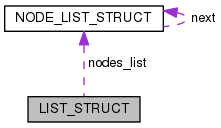
\includegraphics[width=238pt]{structLIST__STRUCT__coll__graph}
\end{center}
\end{figure}
\subsection*{Public Attributes}
\begin{DoxyCompactItemize}
\item 
\hyperlink{DataDefinition_8h_a8804182fdd4652d904801ac03e3d9307}{N\-O\-D\-E\-\_\-\-L\-I\-S\-T} $\ast$ \hyperlink{structLIST__STRUCT_a480f01d85e0c69f63eeeb62c4378e19e}{nodes\-\_\-list}
\end{DoxyCompactItemize}


\subsection{Member Data Documentation}
\hypertarget{structLIST__STRUCT_a480f01d85e0c69f63eeeb62c4378e19e}{\index{L\-I\-S\-T\-\_\-\-S\-T\-R\-U\-C\-T@{L\-I\-S\-T\-\_\-\-S\-T\-R\-U\-C\-T}!nodes\-\_\-list@{nodes\-\_\-list}}
\index{nodes\-\_\-list@{nodes\-\_\-list}!LIST_STRUCT@{L\-I\-S\-T\-\_\-\-S\-T\-R\-U\-C\-T}}
\subsubsection[{nodes\-\_\-list}]{\setlength{\rightskip}{0pt plus 5cm}{\bf N\-O\-D\-E\-\_\-\-L\-I\-S\-T}$\ast$ L\-I\-S\-T\-\_\-\-S\-T\-R\-U\-C\-T\-::nodes\-\_\-list}}\label{structLIST__STRUCT_a480f01d85e0c69f63eeeb62c4378e19e}


The documentation for this struct was generated from the following file\-:\begin{DoxyCompactItemize}
\item 
\hyperlink{DataDefinition_8h}{Data\-Definition.\-h}\end{DoxyCompactItemize}

\hypertarget{structNODE__LIST__STRUCT}{\section{N\-O\-D\-E\-\_\-\-L\-I\-S\-T\-\_\-\-S\-T\-R\-U\-C\-T Struct Reference}
\label{structNODE__LIST__STRUCT}\index{N\-O\-D\-E\-\_\-\-L\-I\-S\-T\-\_\-\-S\-T\-R\-U\-C\-T@{N\-O\-D\-E\-\_\-\-L\-I\-S\-T\-\_\-\-S\-T\-R\-U\-C\-T}}
}


{\ttfamily \#include $<$Data\-Definition.\-h$>$}



Collaboration diagram for N\-O\-D\-E\-\_\-\-L\-I\-S\-T\-\_\-\-S\-T\-R\-U\-C\-T\-:
\nopagebreak
\begin{figure}[H]
\begin{center}
\leavevmode
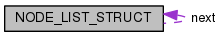
\includegraphics[width=238pt]{structNODE__LIST__STRUCT__coll__graph}
\end{center}
\end{figure}
\subsection*{Public Attributes}
\begin{DoxyCompactItemize}
\item 
int \hyperlink{structNODE__LIST__STRUCT_a34444a74455d1e7d59e13f1dae754321}{id}
\item 
int \hyperlink{structNODE__LIST__STRUCT_a63170b40e99791988837be24d177f65b}{degree}
\item 
int \hyperlink{structNODE__LIST__STRUCT_a5887adfa6a4a3b94ba786593a12fa7ad}{id\-\_\-utente}
\item 
int \hyperlink{structNODE__LIST__STRUCT_abc43d88cc9b8427972095a4637969389}{id\-\_\-file}
\item 
int \hyperlink{structNODE__LIST__STRUCT_a19a415b69b3c7eb1ddeca6ce76670af9}{id\-\_\-chunck}
\item 
struct \hyperlink{structNODE__LIST__STRUCT}{N\-O\-D\-E\-\_\-\-L\-I\-S\-T\-\_\-\-S\-T\-R\-U\-C\-T} $\ast$ \hyperlink{structNODE__LIST__STRUCT_a16cafa75205cd9acf5039b4502613f1a}{next}
\end{DoxyCompactItemize}


\subsection{Member Data Documentation}
\hypertarget{structNODE__LIST__STRUCT_a63170b40e99791988837be24d177f65b}{\index{N\-O\-D\-E\-\_\-\-L\-I\-S\-T\-\_\-\-S\-T\-R\-U\-C\-T@{N\-O\-D\-E\-\_\-\-L\-I\-S\-T\-\_\-\-S\-T\-R\-U\-C\-T}!degree@{degree}}
\index{degree@{degree}!NODE_LIST_STRUCT@{N\-O\-D\-E\-\_\-\-L\-I\-S\-T\-\_\-\-S\-T\-R\-U\-C\-T}}
\subsubsection[{degree}]{\setlength{\rightskip}{0pt plus 5cm}int N\-O\-D\-E\-\_\-\-L\-I\-S\-T\-\_\-\-S\-T\-R\-U\-C\-T\-::degree}}\label{structNODE__LIST__STRUCT_a63170b40e99791988837be24d177f65b}
\hypertarget{structNODE__LIST__STRUCT_a34444a74455d1e7d59e13f1dae754321}{\index{N\-O\-D\-E\-\_\-\-L\-I\-S\-T\-\_\-\-S\-T\-R\-U\-C\-T@{N\-O\-D\-E\-\_\-\-L\-I\-S\-T\-\_\-\-S\-T\-R\-U\-C\-T}!id@{id}}
\index{id@{id}!NODE_LIST_STRUCT@{N\-O\-D\-E\-\_\-\-L\-I\-S\-T\-\_\-\-S\-T\-R\-U\-C\-T}}
\subsubsection[{id}]{\setlength{\rightskip}{0pt plus 5cm}int N\-O\-D\-E\-\_\-\-L\-I\-S\-T\-\_\-\-S\-T\-R\-U\-C\-T\-::id}}\label{structNODE__LIST__STRUCT_a34444a74455d1e7d59e13f1dae754321}
\hypertarget{structNODE__LIST__STRUCT_a19a415b69b3c7eb1ddeca6ce76670af9}{\index{N\-O\-D\-E\-\_\-\-L\-I\-S\-T\-\_\-\-S\-T\-R\-U\-C\-T@{N\-O\-D\-E\-\_\-\-L\-I\-S\-T\-\_\-\-S\-T\-R\-U\-C\-T}!id\-\_\-chunck@{id\-\_\-chunck}}
\index{id\-\_\-chunck@{id\-\_\-chunck}!NODE_LIST_STRUCT@{N\-O\-D\-E\-\_\-\-L\-I\-S\-T\-\_\-\-S\-T\-R\-U\-C\-T}}
\subsubsection[{id\-\_\-chunck}]{\setlength{\rightskip}{0pt plus 5cm}int N\-O\-D\-E\-\_\-\-L\-I\-S\-T\-\_\-\-S\-T\-R\-U\-C\-T\-::id\-\_\-chunck}}\label{structNODE__LIST__STRUCT_a19a415b69b3c7eb1ddeca6ce76670af9}
\hypertarget{structNODE__LIST__STRUCT_abc43d88cc9b8427972095a4637969389}{\index{N\-O\-D\-E\-\_\-\-L\-I\-S\-T\-\_\-\-S\-T\-R\-U\-C\-T@{N\-O\-D\-E\-\_\-\-L\-I\-S\-T\-\_\-\-S\-T\-R\-U\-C\-T}!id\-\_\-file@{id\-\_\-file}}
\index{id\-\_\-file@{id\-\_\-file}!NODE_LIST_STRUCT@{N\-O\-D\-E\-\_\-\-L\-I\-S\-T\-\_\-\-S\-T\-R\-U\-C\-T}}
\subsubsection[{id\-\_\-file}]{\setlength{\rightskip}{0pt plus 5cm}int N\-O\-D\-E\-\_\-\-L\-I\-S\-T\-\_\-\-S\-T\-R\-U\-C\-T\-::id\-\_\-file}}\label{structNODE__LIST__STRUCT_abc43d88cc9b8427972095a4637969389}
\hypertarget{structNODE__LIST__STRUCT_a5887adfa6a4a3b94ba786593a12fa7ad}{\index{N\-O\-D\-E\-\_\-\-L\-I\-S\-T\-\_\-\-S\-T\-R\-U\-C\-T@{N\-O\-D\-E\-\_\-\-L\-I\-S\-T\-\_\-\-S\-T\-R\-U\-C\-T}!id\-\_\-utente@{id\-\_\-utente}}
\index{id\-\_\-utente@{id\-\_\-utente}!NODE_LIST_STRUCT@{N\-O\-D\-E\-\_\-\-L\-I\-S\-T\-\_\-\-S\-T\-R\-U\-C\-T}}
\subsubsection[{id\-\_\-utente}]{\setlength{\rightskip}{0pt plus 5cm}int N\-O\-D\-E\-\_\-\-L\-I\-S\-T\-\_\-\-S\-T\-R\-U\-C\-T\-::id\-\_\-utente}}\label{structNODE__LIST__STRUCT_a5887adfa6a4a3b94ba786593a12fa7ad}
\hypertarget{structNODE__LIST__STRUCT_a16cafa75205cd9acf5039b4502613f1a}{\index{N\-O\-D\-E\-\_\-\-L\-I\-S\-T\-\_\-\-S\-T\-R\-U\-C\-T@{N\-O\-D\-E\-\_\-\-L\-I\-S\-T\-\_\-\-S\-T\-R\-U\-C\-T}!next@{next}}
\index{next@{next}!NODE_LIST_STRUCT@{N\-O\-D\-E\-\_\-\-L\-I\-S\-T\-\_\-\-S\-T\-R\-U\-C\-T}}
\subsubsection[{next}]{\setlength{\rightskip}{0pt plus 5cm}struct {\bf N\-O\-D\-E\-\_\-\-L\-I\-S\-T\-\_\-\-S\-T\-R\-U\-C\-T}$\ast$ N\-O\-D\-E\-\_\-\-L\-I\-S\-T\-\_\-\-S\-T\-R\-U\-C\-T\-::next}}\label{structNODE__LIST__STRUCT_a16cafa75205cd9acf5039b4502613f1a}


The documentation for this struct was generated from the following file\-:\begin{DoxyCompactItemize}
\item 
\hyperlink{DataDefinition_8h}{Data\-Definition.\-h}\end{DoxyCompactItemize}

\hypertarget{structNODE__STRUCT}{\section{N\-O\-D\-E\-\_\-\-S\-T\-R\-U\-C\-T Struct Reference}
\label{structNODE__STRUCT}\index{N\-O\-D\-E\-\_\-\-S\-T\-R\-U\-C\-T@{N\-O\-D\-E\-\_\-\-S\-T\-R\-U\-C\-T}}
}


{\ttfamily \#include $<$Data\-Definition.\-h$>$}



Collaboration diagram for N\-O\-D\-E\-\_\-\-S\-T\-R\-U\-C\-T\-:
\nopagebreak
\begin{figure}[H]
\begin{center}
\leavevmode
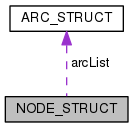
\includegraphics[width=172pt]{structNODE__STRUCT__coll__graph}
\end{center}
\end{figure}
\subsection*{Public Attributes}
\begin{DoxyCompactItemize}
\item 
int \hyperlink{structNODE__STRUCT_a4386a981b07860b03b46d11c5280445d}{id}
\item 
int \hyperlink{structNODE__STRUCT_a4d119525d60341ec5fb1c0f040adb867}{degree}
\item 
struct \hyperlink{structARC__STRUCT}{A\-R\-C\-\_\-\-S\-T\-R\-U\-C\-T} $\ast$ \hyperlink{structNODE__STRUCT_a0a9adf25cd6c875ce28817790e2d93f7}{arc\-List}
\end{DoxyCompactItemize}


\subsection{Member Data Documentation}
\hypertarget{structNODE__STRUCT_a0a9adf25cd6c875ce28817790e2d93f7}{\index{N\-O\-D\-E\-\_\-\-S\-T\-R\-U\-C\-T@{N\-O\-D\-E\-\_\-\-S\-T\-R\-U\-C\-T}!arc\-List@{arc\-List}}
\index{arc\-List@{arc\-List}!NODE_STRUCT@{N\-O\-D\-E\-\_\-\-S\-T\-R\-U\-C\-T}}
\subsubsection[{arc\-List}]{\setlength{\rightskip}{0pt plus 5cm}struct {\bf A\-R\-C\-\_\-\-S\-T\-R\-U\-C\-T}$\ast$ N\-O\-D\-E\-\_\-\-S\-T\-R\-U\-C\-T\-::arc\-List}}\label{structNODE__STRUCT_a0a9adf25cd6c875ce28817790e2d93f7}
\hypertarget{structNODE__STRUCT_a4d119525d60341ec5fb1c0f040adb867}{\index{N\-O\-D\-E\-\_\-\-S\-T\-R\-U\-C\-T@{N\-O\-D\-E\-\_\-\-S\-T\-R\-U\-C\-T}!degree@{degree}}
\index{degree@{degree}!NODE_STRUCT@{N\-O\-D\-E\-\_\-\-S\-T\-R\-U\-C\-T}}
\subsubsection[{degree}]{\setlength{\rightskip}{0pt plus 5cm}int N\-O\-D\-E\-\_\-\-S\-T\-R\-U\-C\-T\-::degree}}\label{structNODE__STRUCT_a4d119525d60341ec5fb1c0f040adb867}
\hypertarget{structNODE__STRUCT_a4386a981b07860b03b46d11c5280445d}{\index{N\-O\-D\-E\-\_\-\-S\-T\-R\-U\-C\-T@{N\-O\-D\-E\-\_\-\-S\-T\-R\-U\-C\-T}!id@{id}}
\index{id@{id}!NODE_STRUCT@{N\-O\-D\-E\-\_\-\-S\-T\-R\-U\-C\-T}}
\subsubsection[{id}]{\setlength{\rightskip}{0pt plus 5cm}int N\-O\-D\-E\-\_\-\-S\-T\-R\-U\-C\-T\-::id}}\label{structNODE__STRUCT_a4386a981b07860b03b46d11c5280445d}


The documentation for this struct was generated from the following file\-:\begin{DoxyCompactItemize}
\item 
\hyperlink{DataDefinition_8h}{Data\-Definition.\-h}\end{DoxyCompactItemize}

\hypertarget{structNODE__SUBSET__STRUCT}{\section{N\-O\-D\-E\-\_\-\-S\-U\-B\-S\-E\-T\-\_\-\-S\-T\-R\-U\-C\-T Struct Reference}
\label{structNODE__SUBSET__STRUCT}\index{N\-O\-D\-E\-\_\-\-S\-U\-B\-S\-E\-T\-\_\-\-S\-T\-R\-U\-C\-T@{N\-O\-D\-E\-\_\-\-S\-U\-B\-S\-E\-T\-\_\-\-S\-T\-R\-U\-C\-T}}
}


{\ttfamily \#include $<$Data\-Definition.\-h$>$}



Collaboration diagram for N\-O\-D\-E\-\_\-\-S\-U\-B\-S\-E\-T\-\_\-\-S\-T\-R\-U\-C\-T\-:
\nopagebreak
\begin{figure}[H]
\begin{center}
\leavevmode
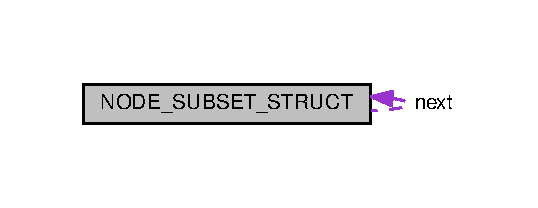
\includegraphics[width=258pt]{structNODE__SUBSET__STRUCT__coll__graph}
\end{center}
\end{figure}
\subsection*{Public Attributes}
\begin{DoxyCompactItemize}
\item 
int \hyperlink{structNODE__SUBSET__STRUCT_a8047d3c37caf8eed1d5cf1db677a6e6a}{id}
\item 
int \hyperlink{structNODE__SUBSET__STRUCT_a8945dd5c7d8177ffbee4acd74ab600d2}{cardinality}
\item 
int $\ast$ \hyperlink{structNODE__SUBSET__STRUCT_a4c704f400a1fa5bb309c1c243422eda1}{label}
\item 
int \hyperlink{structNODE__SUBSET__STRUCT_ab2b2587d1db1672a8dcf6e7050b30f82}{size\-\_\-label}
\item 
struct \hyperlink{structNODE__SUBSET__STRUCT}{N\-O\-D\-E\-\_\-\-S\-U\-B\-S\-E\-T\-\_\-\-S\-T\-R\-U\-C\-T} $\ast$ \hyperlink{structNODE__SUBSET__STRUCT_a23d8738ae1b4513d607523d289e40ace}{next}
\end{DoxyCompactItemize}


\subsection{Member Data Documentation}
\hypertarget{structNODE__SUBSET__STRUCT_a8945dd5c7d8177ffbee4acd74ab600d2}{\index{N\-O\-D\-E\-\_\-\-S\-U\-B\-S\-E\-T\-\_\-\-S\-T\-R\-U\-C\-T@{N\-O\-D\-E\-\_\-\-S\-U\-B\-S\-E\-T\-\_\-\-S\-T\-R\-U\-C\-T}!cardinality@{cardinality}}
\index{cardinality@{cardinality}!NODE_SUBSET_STRUCT@{N\-O\-D\-E\-\_\-\-S\-U\-B\-S\-E\-T\-\_\-\-S\-T\-R\-U\-C\-T}}
\subsubsection[{cardinality}]{\setlength{\rightskip}{0pt plus 5cm}int N\-O\-D\-E\-\_\-\-S\-U\-B\-S\-E\-T\-\_\-\-S\-T\-R\-U\-C\-T\-::cardinality}}\label{structNODE__SUBSET__STRUCT_a8945dd5c7d8177ffbee4acd74ab600d2}
\hypertarget{structNODE__SUBSET__STRUCT_a8047d3c37caf8eed1d5cf1db677a6e6a}{\index{N\-O\-D\-E\-\_\-\-S\-U\-B\-S\-E\-T\-\_\-\-S\-T\-R\-U\-C\-T@{N\-O\-D\-E\-\_\-\-S\-U\-B\-S\-E\-T\-\_\-\-S\-T\-R\-U\-C\-T}!id@{id}}
\index{id@{id}!NODE_SUBSET_STRUCT@{N\-O\-D\-E\-\_\-\-S\-U\-B\-S\-E\-T\-\_\-\-S\-T\-R\-U\-C\-T}}
\subsubsection[{id}]{\setlength{\rightskip}{0pt plus 5cm}int N\-O\-D\-E\-\_\-\-S\-U\-B\-S\-E\-T\-\_\-\-S\-T\-R\-U\-C\-T\-::id}}\label{structNODE__SUBSET__STRUCT_a8047d3c37caf8eed1d5cf1db677a6e6a}
\hypertarget{structNODE__SUBSET__STRUCT_a4c704f400a1fa5bb309c1c243422eda1}{\index{N\-O\-D\-E\-\_\-\-S\-U\-B\-S\-E\-T\-\_\-\-S\-T\-R\-U\-C\-T@{N\-O\-D\-E\-\_\-\-S\-U\-B\-S\-E\-T\-\_\-\-S\-T\-R\-U\-C\-T}!label@{label}}
\index{label@{label}!NODE_SUBSET_STRUCT@{N\-O\-D\-E\-\_\-\-S\-U\-B\-S\-E\-T\-\_\-\-S\-T\-R\-U\-C\-T}}
\subsubsection[{label}]{\setlength{\rightskip}{0pt plus 5cm}int$\ast$ N\-O\-D\-E\-\_\-\-S\-U\-B\-S\-E\-T\-\_\-\-S\-T\-R\-U\-C\-T\-::label}}\label{structNODE__SUBSET__STRUCT_a4c704f400a1fa5bb309c1c243422eda1}
\hypertarget{structNODE__SUBSET__STRUCT_a23d8738ae1b4513d607523d289e40ace}{\index{N\-O\-D\-E\-\_\-\-S\-U\-B\-S\-E\-T\-\_\-\-S\-T\-R\-U\-C\-T@{N\-O\-D\-E\-\_\-\-S\-U\-B\-S\-E\-T\-\_\-\-S\-T\-R\-U\-C\-T}!next@{next}}
\index{next@{next}!NODE_SUBSET_STRUCT@{N\-O\-D\-E\-\_\-\-S\-U\-B\-S\-E\-T\-\_\-\-S\-T\-R\-U\-C\-T}}
\subsubsection[{next}]{\setlength{\rightskip}{0pt plus 5cm}struct {\bf N\-O\-D\-E\-\_\-\-S\-U\-B\-S\-E\-T\-\_\-\-S\-T\-R\-U\-C\-T}$\ast$ N\-O\-D\-E\-\_\-\-S\-U\-B\-S\-E\-T\-\_\-\-S\-T\-R\-U\-C\-T\-::next}}\label{structNODE__SUBSET__STRUCT_a23d8738ae1b4513d607523d289e40ace}
\hypertarget{structNODE__SUBSET__STRUCT_ab2b2587d1db1672a8dcf6e7050b30f82}{\index{N\-O\-D\-E\-\_\-\-S\-U\-B\-S\-E\-T\-\_\-\-S\-T\-R\-U\-C\-T@{N\-O\-D\-E\-\_\-\-S\-U\-B\-S\-E\-T\-\_\-\-S\-T\-R\-U\-C\-T}!size\-\_\-label@{size\-\_\-label}}
\index{size\-\_\-label@{size\-\_\-label}!NODE_SUBSET_STRUCT@{N\-O\-D\-E\-\_\-\-S\-U\-B\-S\-E\-T\-\_\-\-S\-T\-R\-U\-C\-T}}
\subsubsection[{size\-\_\-label}]{\setlength{\rightskip}{0pt plus 5cm}int N\-O\-D\-E\-\_\-\-S\-U\-B\-S\-E\-T\-\_\-\-S\-T\-R\-U\-C\-T\-::size\-\_\-label}}\label{structNODE__SUBSET__STRUCT_ab2b2587d1db1672a8dcf6e7050b30f82}


The documentation for this struct was generated from the following file\-:\begin{DoxyCompactItemize}
\item 
\hyperlink{DataDefinition_8h}{Data\-Definition.\-h}\end{DoxyCompactItemize}

\hypertarget{structNODO}{\section{N\-O\-D\-O Struct Reference}
\label{structNODO}\index{N\-O\-D\-O@{N\-O\-D\-O}}
}
\subsection*{Public Attributes}
\begin{DoxyCompactItemize}
\item 
\hypertarget{structNODO_a363311f2eac0f019bb559decee9d283a}{int {\bfseries id}}\label{structNODO_a363311f2eac0f019bb559decee9d283a}

\item 
\hypertarget{structNODO_ac347f94dfc5042c7a35b5a2ae30796c3}{int {\bfseries degree}}\label{structNODO_ac347f94dfc5042c7a35b5a2ae30796c3}

\item 
\hypertarget{structNODO_a3d58b6fffbdc9fa4dd781d6e5d775ce5}{int {\bfseries id\-\_\-utente}}\label{structNODO_a3d58b6fffbdc9fa4dd781d6e5d775ce5}

\item 
\hypertarget{structNODO_ad1f3355d97fd04e0d908dc196bbf07af}{int {\bfseries id\-\_\-file}}\label{structNODO_ad1f3355d97fd04e0d908dc196bbf07af}

\item 
\hypertarget{structNODO_afff09f10bea60ea56ef2ee708a876017}{int {\bfseries id\-\_\-chunck}}\label{structNODO_afff09f10bea60ea56ef2ee708a876017}

\end{DoxyCompactItemize}


The documentation for this struct was generated from the following file\-:\begin{DoxyCompactItemize}
\item 
Data\-Definition.\-h\end{DoxyCompactItemize}

\hypertarget{structRANDOM__LIST}{\section{R\-A\-N\-D\-O\-M\-\_\-\-L\-I\-S\-T Struct Reference}
\label{structRANDOM__LIST}\index{R\-A\-N\-D\-O\-M\-\_\-\-L\-I\-S\-T@{R\-A\-N\-D\-O\-M\-\_\-\-L\-I\-S\-T}}
}
\subsection*{Public Attributes}
\begin{DoxyCompactItemize}
\item 
\hypertarget{structRANDOM__LIST_a6cd2e0e1e170a5692dc48a4d4c87bdc6}{int {\bfseries idx}}\label{structRANDOM__LIST_a6cd2e0e1e170a5692dc48a4d4c87bdc6}

\item 
\hypertarget{structRANDOM__LIST_a69d18749d83881f09a2742cd6ba19d28}{struct \hyperlink{structRANDOM__LIST}{R\-A\-N\-D\-O\-M\-\_\-\-L\-I\-S\-T} $\ast$ {\bfseries next}}\label{structRANDOM__LIST_a69d18749d83881f09a2742cd6ba19d28}

\end{DoxyCompactItemize}


The documentation for this struct was generated from the following file\-:\begin{DoxyCompactItemize}
\item 
Data\-Definition.\-h\end{DoxyCompactItemize}

\hypertarget{structRCL__LIST__STRUCT}{\section{R\-C\-L\-\_\-\-L\-I\-S\-T\-\_\-\-S\-T\-R\-U\-C\-T Struct Reference}
\label{structRCL__LIST__STRUCT}\index{R\-C\-L\-\_\-\-L\-I\-S\-T\-\_\-\-S\-T\-R\-U\-C\-T@{R\-C\-L\-\_\-\-L\-I\-S\-T\-\_\-\-S\-T\-R\-U\-C\-T}}
}


{\ttfamily \#include $<$Data\-Definition.\-h$>$}

\subsection*{Public Attributes}
\begin{DoxyCompactItemize}
\item 
int \hyperlink{structRCL__LIST__STRUCT_a1fe9da973a851dad04eb6b0272b35adb}{i}
\end{DoxyCompactItemize}


\subsection{Member Data Documentation}
\hypertarget{structRCL__LIST__STRUCT_a1fe9da973a851dad04eb6b0272b35adb}{\index{R\-C\-L\-\_\-\-L\-I\-S\-T\-\_\-\-S\-T\-R\-U\-C\-T@{R\-C\-L\-\_\-\-L\-I\-S\-T\-\_\-\-S\-T\-R\-U\-C\-T}!i@{i}}
\index{i@{i}!RCL_LIST_STRUCT@{R\-C\-L\-\_\-\-L\-I\-S\-T\-\_\-\-S\-T\-R\-U\-C\-T}}
\subsubsection[{i}]{\setlength{\rightskip}{0pt plus 5cm}int R\-C\-L\-\_\-\-L\-I\-S\-T\-\_\-\-S\-T\-R\-U\-C\-T\-::i}}\label{structRCL__LIST__STRUCT_a1fe9da973a851dad04eb6b0272b35adb}


The documentation for this struct was generated from the following file\-:\begin{DoxyCompactItemize}
\item 
\hyperlink{DataDefinition_8h}{Data\-Definition.\-h}\end{DoxyCompactItemize}

\hypertarget{structSUBSET__STRUCT}{\section{S\-U\-B\-S\-E\-T\-\_\-\-S\-T\-R\-U\-C\-T Struct Reference}
\label{structSUBSET__STRUCT}\index{S\-U\-B\-S\-E\-T\-\_\-\-S\-T\-R\-U\-C\-T@{S\-U\-B\-S\-E\-T\-\_\-\-S\-T\-R\-U\-C\-T}}
}
\subsection*{Public Attributes}
\begin{DoxyCompactItemize}
\item 
\hypertarget{structSUBSET__STRUCT_a8023cbde4ffe195b6fa3fd9a7c3211f6}{\hyperlink{structNODE__SUBSET__STRUCT}{N\-O\-D\-E\-\_\-\-S\-U\-B\-S\-E\-T} $\ast$ {\bfseries pt\-\_\-end}}\label{structSUBSET__STRUCT_a8023cbde4ffe195b6fa3fd9a7c3211f6}

\item 
\hypertarget{structSUBSET__STRUCT_a61f3350ae28b746fea56129536e73ec1}{\hyperlink{structNODE__SUBSET__STRUCT}{N\-O\-D\-E\-\_\-\-S\-U\-B\-S\-E\-T} $\ast$ {\bfseries nodes\-\_\-list}}\label{structSUBSET__STRUCT_a61f3350ae28b746fea56129536e73ec1}

\end{DoxyCompactItemize}


The documentation for this struct was generated from the following file\-:\begin{DoxyCompactItemize}
\item 
Data\-Definition.\-h\end{DoxyCompactItemize}

\chapter{File Documentation}
\hypertarget{client_8cpp}{\section{client.\-cpp File Reference}
\label{client_8cpp}\index{client.\-cpp@{client.\-cpp}}
}


The main file to use the client.  


{\ttfamily \#include \char`\"{}Coding\-Decoding\-Data.\-h\char`\"{}}\\*
{\ttfamily \#include \char`\"{}Lib\-Shine.\-h\char`\"{}}\\*
{\ttfamily \#include $<$arpa/inet.\-h$>$}\\*
{\ttfamily \#include $<$cstring$>$}\\*
{\ttfamily \#include $<$unistd.\-h$>$}\\*
{\ttfamily \#include $<$netdb.\-h$>$}\\*
{\ttfamily \#include $<$sys/types.\-h$>$}\\*
\subsection*{Macros}
\begin{DoxyCompactItemize}
\item 
\hypertarget{client_8cpp_a06a4f92382a282853f27039c63fb0c91}{\#define {\bfseries H\-E\-L\-L\-O\-\_\-\-P\-O\-R\-T}~12345}\label{client_8cpp_a06a4f92382a282853f27039c63fb0c91}

\item 
\hypertarget{client_8cpp_aa869892c2393564caaf8c65af8225e6b}{\#define {\bfseries H\-E\-L\-L\-O\-\_\-\-G\-R\-O\-U\-P}~\char`\"{}225.\-0.\-0.\-37\char`\"{}}\label{client_8cpp_aa869892c2393564caaf8c65af8225e6b}

\item 
\hypertarget{client_8cpp_aad9be19ed0c1f5871c9932df83023026}{\#define {\bfseries M\-S\-G\-B\-U\-F\-S\-I\-Z\-E}~1024}\label{client_8cpp_aad9be19ed0c1f5871c9932df83023026}

\end{DoxyCompactItemize}
\subsection*{Functions}
\begin{DoxyCompactItemize}
\item 
void $\ast$ \hyperlink{client_8cpp_ab831c44f8ddb7ea2b41ada3f8c263d80}{task\-Udp} (void $\ast$)
\item 
int \hyperlink{client_8cpp_a0ddf1224851353fc92bfbff6f499fa97}{main} (int argc, char $\ast$argv\mbox{[}$\,$\mbox{]})
\end{DoxyCompactItemize}
\subsection*{Variables}
\begin{DoxyCompactItemize}
\item 
\hypertarget{client_8cpp_aa9a265bfabda02a49e53d82a904308e1}{pthread\-\_\-t {\bfseries thread\-A} \mbox{[}3\mbox{]}}\label{client_8cpp_aa9a265bfabda02a49e53d82a904308e1}

\item 
\hypertarget{client_8cpp_a939bd384596ea8e992d652270a133b55}{vector$<$ char $>$ {\bfseries coded\-\_\-data}}\label{client_8cpp_a939bd384596ea8e992d652270a133b55}

\item 
\hypertarget{client_8cpp_a1e1e165e89d4b4809ccbbe7aada77077}{\hyperlink{structHEADER__TRANSMISSION}{header\-\_\-transmission} {\bfseries header}}\label{client_8cpp_a1e1e165e89d4b4809ccbbe7aada77077}

\item 
\hypertarget{client_8cpp_afc67ef5edf9d0bc08795a14a07d8633c}{int {\bfseries id\-\_\-requested\-\_\-file} = -\/I\-N\-F}\label{client_8cpp_afc67ef5edf9d0bc08795a14a07d8633c}

\item 
\hypertarget{client_8cpp_a2083d0af7adbc4404b62ae6786b96f20}{int {\bfseries id\-\_\-utente} =0}\label{client_8cpp_a2083d0af7adbc4404b62ae6786b96f20}

\item 
\hyperlink{structConfig}{Config} \hyperlink{client_8cpp_a4a8dd3a2de125b72d4fe6251a0a271b5}{config}
\item 
\hypertarget{client_8cpp_a36dadae3093227b3e1c48a749e0c2d68}{log4cpp\-::\-Appender $\ast$ {\bfseries appender1}}\label{client_8cpp_a36dadae3093227b3e1c48a749e0c2d68}

\item 
\hypertarget{client_8cpp_a65af033419450d60618533fde8ab81b0}{log4cpp\-::\-Category \& {\bfseries root} = log4cpp\-::\-Category\-::get\-Root()}\label{client_8cpp_a65af033419450d60618533fde8ab81b0}

\end{DoxyCompactItemize}


\subsection{Detailed Description}
The main file to use the client. 

\subsection{Function Documentation}
\hypertarget{client_8cpp_a0ddf1224851353fc92bfbff6f499fa97}{\index{client.\-cpp@{client.\-cpp}!main@{main}}
\index{main@{main}!client.cpp@{client.\-cpp}}
\subsubsection[{main}]{\setlength{\rightskip}{0pt plus 5cm}int main (
\begin{DoxyParamCaption}
\item[{int}]{argc, }
\item[{char $\ast$}]{argv\mbox{[}$\,$\mbox{]}}
\end{DoxyParamCaption}
)}}\label{client_8cpp_a0ddf1224851353fc92bfbff6f499fa97}
main function this function open a T\-C\-P connection to the server and run a thread to Listen U\-D\-P \hypertarget{client_8cpp_ab831c44f8ddb7ea2b41ada3f8c263d80}{\index{client.\-cpp@{client.\-cpp}!task\-Udp@{task\-Udp}}
\index{task\-Udp@{task\-Udp}!client.cpp@{client.\-cpp}}
\subsubsection[{task\-Udp}]{\setlength{\rightskip}{0pt plus 5cm}void $\ast$ task\-Udp (
\begin{DoxyParamCaption}
\item[{void $\ast$}]{prt}
\end{DoxyParamCaption}
)}}\label{client_8cpp_ab831c44f8ddb7ea2b41ada3f8c263d80}
Thread for recive data. This thread open a U\-D\-P connection for listen U\-D\-P and are executed the algorithms to decode and save data. 

\subsection{Variable Documentation}
\hypertarget{client_8cpp_a4a8dd3a2de125b72d4fe6251a0a271b5}{\index{client.\-cpp@{client.\-cpp}!config@{config}}
\index{config@{config}!client.cpp@{client.\-cpp}}
\subsubsection[{config}]{\setlength{\rightskip}{0pt plus 5cm}{\bf Config} config}}\label{client_8cpp_a4a8dd3a2de125b72d4fe6251a0a271b5}
Struct for loading configuration file .ini 
\hypertarget{CodingDecodingData_8cpp}{\section{Coding\-Decoding\-Data.\-cpp File Reference}
\label{CodingDecodingData_8cpp}\index{Coding\-Decoding\-Data.\-cpp@{Coding\-Decoding\-Data.\-cpp}}
}


The file that perform the decoding.  


{\ttfamily \#include \char`\"{}Coding\-Decoding\-Data.\-h\char`\"{}}\\*
{\ttfamily \#include $<$cstring$>$}\\*
\subsection*{Functions}
\begin{DoxyCompactItemize}
\item 
void \hyperlink{CodingDecodingData_8cpp_ace3496fe483a779146e070625c0435b4}{decoding\-Data} (\hyperlink{structHEADER__TRANSMISSION}{header\-\_\-transmission} header, vector$<$ char $>$ \&coded\-\_\-data, int m\-\_\-files, int id\-\_\-utente, int id\-\_\-requested\-\_\-file, string path\-Folder)
\end{DoxyCompactItemize}


\subsection{Detailed Description}
The file that perform the decoding. 

\subsection{Function Documentation}
\hypertarget{CodingDecodingData_8cpp_ace3496fe483a779146e070625c0435b4}{\index{Coding\-Decoding\-Data.\-cpp@{Coding\-Decoding\-Data.\-cpp}!decoding\-Data@{decoding\-Data}}
\index{decoding\-Data@{decoding\-Data}!CodingDecodingData.cpp@{Coding\-Decoding\-Data.\-cpp}}
\subsubsection[{decoding\-Data}]{\setlength{\rightskip}{0pt plus 5cm}void decoding\-Data (
\begin{DoxyParamCaption}
\item[{{\bf header\-\_\-transmission}}]{header, }
\item[{vector$<$ char $>$ \&}]{coded\-\_\-data, }
\item[{int}]{m\-\_\-files, }
\item[{int}]{id\-\_\-utente, }
\item[{int}]{id\-\_\-requested\-\_\-file, }
\item[{string}]{path\-Folder}
\end{DoxyParamCaption}
)}}\label{CodingDecodingData_8cpp_ace3496fe483a779146e070625c0435b4}
function to decode and save the data 
\hypertarget{LibShine_8cpp}{\section{Lib\-Shine.\-cpp File Reference}
\label{LibShine_8cpp}\index{Lib\-Shine.\-cpp@{Lib\-Shine.\-cpp}}
}


The file to load configuration file.  


{\ttfamily \#include \char`\"{}Lib\-Shine.\-h\char`\"{}}\\*
\subsection*{Functions}
\begin{DoxyCompactItemize}
\item 
\hypertarget{LibShine_8cpp_a1539653d5372a4a41b82f85018b99fdf}{void {\bfseries load\-Config\-File} (\hyperlink{structConfig}{Config} \&\hyperlink{client_8cpp_a4a8dd3a2de125b72d4fe6251a0a271b5}{config})}\label{LibShine_8cpp_a1539653d5372a4a41b82f85018b99fdf}

\end{DoxyCompactItemize}


\subsection{Detailed Description}
The file to load configuration file. 
\hypertarget{utilityForTesting_8cpp}{\section{utility\-For\-Testing.\-cpp File Reference}
\label{utilityForTesting_8cpp}\index{utility\-For\-Testing.\-cpp@{utility\-For\-Testing.\-cpp}}
}


A file containing utility function.  


{\ttfamily \#include \char`\"{}utility\-For\-Testing.\-h\char`\"{}}\\*
Include dependency graph for utility\-For\-Testing.\-cpp\-:
\nopagebreak
\begin{figure}[H]
\begin{center}
\leavevmode
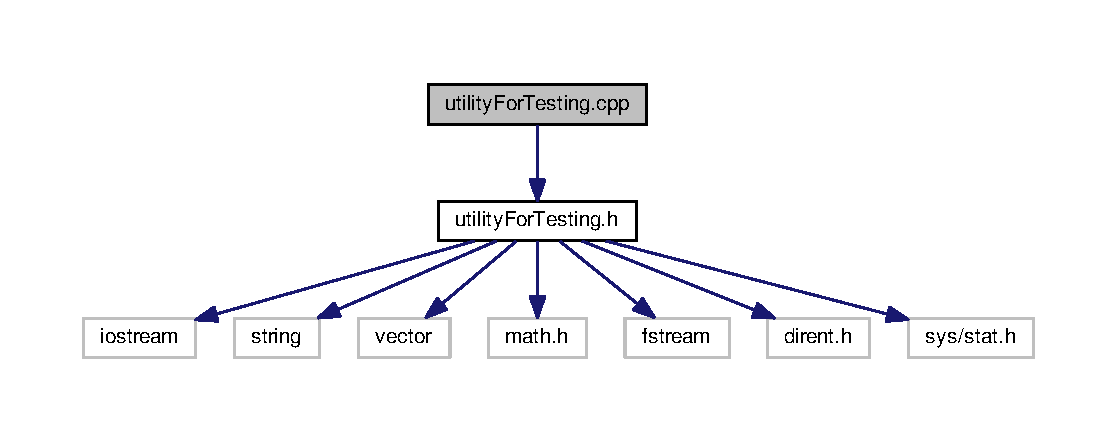
\includegraphics[width=350pt]{utilityForTesting_8cpp__incl}
\end{center}
\end{figure}
\subsection*{Functions}
\begin{DoxyCompactItemize}
\item 
vector$<$ string $>$ \hyperlink{utilityForTesting_8cpp_aa99bf5bbc2250122222555c8aca88f18}{get\-Directory\-Files} (string \&directory)
\end{DoxyCompactItemize}


\subsection{Detailed Description}
A file containing utility function. 

\subsection{Function Documentation}
\hypertarget{utilityForTesting_8cpp_aa99bf5bbc2250122222555c8aca88f18}{\index{utility\-For\-Testing.\-cpp@{utility\-For\-Testing.\-cpp}!get\-Directory\-Files@{get\-Directory\-Files}}
\index{get\-Directory\-Files@{get\-Directory\-Files}!utilityForTesting.cpp@{utility\-For\-Testing.\-cpp}}
\subsubsection[{get\-Directory\-Files}]{\setlength{\rightskip}{0pt plus 5cm}vector$<$string$>$ get\-Directory\-Files (
\begin{DoxyParamCaption}
\item[{string \&}]{directory}
\end{DoxyParamCaption}
)}}\label{utilityForTesting_8cpp_aa99bf5bbc2250122222555c8aca88f18}
function to get a vector of files contained in a directory 

Here is the caller graph for this function\-:
\nopagebreak
\begin{figure}[H]
\begin{center}
\leavevmode
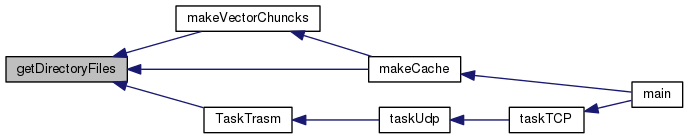
\includegraphics[width=350pt]{utilityForTesting_8cpp_aa99bf5bbc2250122222555c8aca88f18_icgraph}
\end{center}
\end{figure}



%--- End generated contents ---

% Index
\newpage
\phantomsection
\addcontentsline{toc}{chapter}{Index}
\printindex

\end{document}
